\chapter{Experiments}

We used two benchmark datasets to compare our techniques to prior work. We followed the pipeline detailed in the prior chapter, and outline the results and analysis here.

An intuitive way to evaluate our methods would be to execute visual odometry, perform training and indexing, and then retrieve poses for each train query. However, the retrieved poses cannot be directly compared to the ground truth poses, because the coordinate frame used during visual odometry is in general not the same as the one from the ground truth. One way to correct this is to compute a similarity transform from visual odometry to ground truth poses. For example, assuming the $i$th ground truth pose has position $\boldsymbol{X}^{\text{GT}}_i$, and corresponds to the $i$th visual odometry pose with position $\boldsymbol{X}^{\text{VO}}_i$, then (ignoring orientation correspondences) we could minimize:

\begin{equation}
(\boldsymbol{R}^*, \boldsymbol{t}^*, s^*) = \argmin_{\boldsymbol{R}, \boldsymbol{t}, s} \sum_i || s(\boldsymbol{R} \boldsymbol{X}^{\text{VO}}_i + \boldsymbol{t}) - \boldsymbol{X}^{\text{GT}}_i||_2^2
\end{equation}

Observe that it is fine to use the (non-robust) L2 norm here, since we assume that every visual odometry pose is close to the true pose. In this form, there exists a closed form solution based on the singular value decomposition (see, for example, \cite{umeyama1991least} for a derivation). However this fails in the case of large drift or, worse, complete tracking failure in the visual odometry poses. In \fref{fig:alignment_failure}, DSO encounters very poor tracking partway through the sequence, and although frame-to-frame tracking persists, it does so in a different reference frame and at a different scale.

\begin{figure}[h]
	\centering
	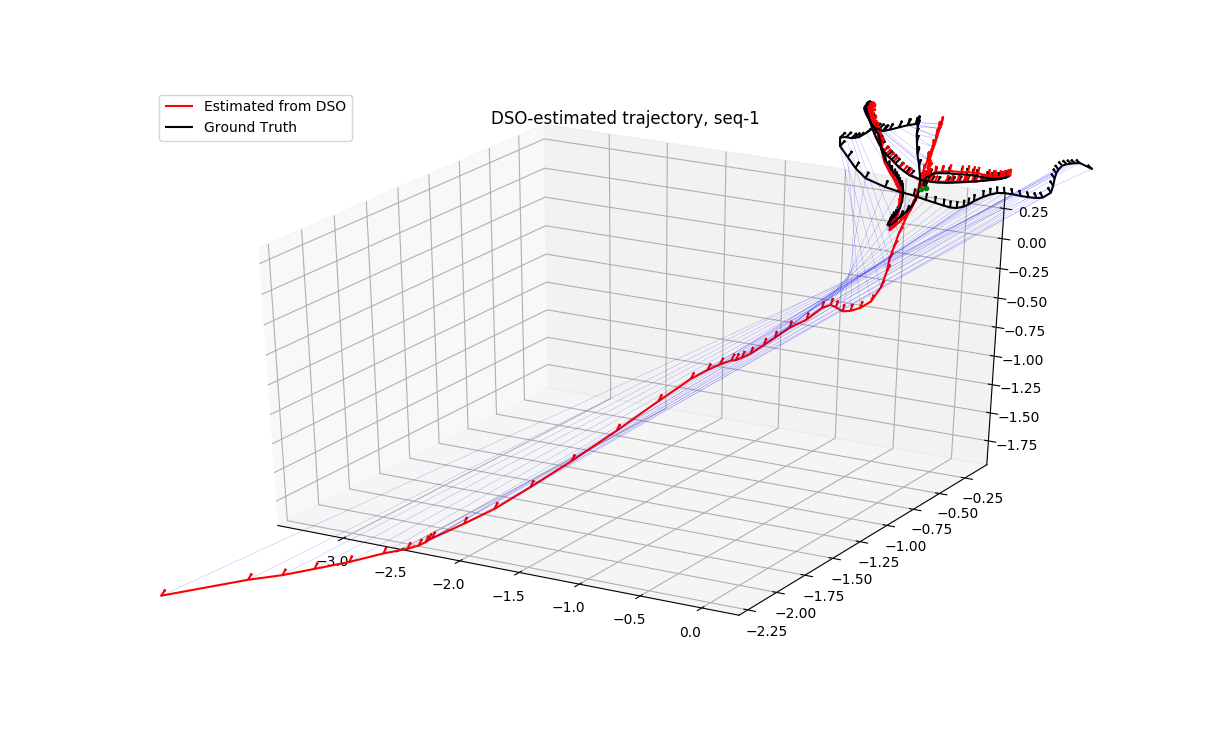
\includegraphics[width=0.8\linewidth]{experiments/alignment_failure.png}
	\caption{Alignment failure between ground truth poses and visual odometry estimated for one sequence from 7-Scenes. Black lines indicate ground truth, red indicates visual odometry, blue lines indicate frame correspondences, and green dots indicate the starting points of the trajectories. Here, a similarity alignment is computed from the first 100 poses; however, the trajectories diverge in the last half of the sequence, making these frames ineffective for relocalization.}
	\label{fig:alignment_failure}
\end{figure}

In a full end-to-end SLAM system, such as LSD-SLAM, it would be desirable to test the ability of the system to recover from tracking failure (by returning to the old reference frame), and to minimize drift over time. However, in our tests, we would like to localize to ground truth measurements provided in the training set, so that our results are comparable to previous relocalization work. Ideally, we would like to minimize drift and even provide a candidate pose in situations where one cannot be estimated by visual odometry with sufficient certainty. Accordingly, we make several changes to DSO. 

The first modification is to the initializer, which determines the initial scale of the reconstruction. We fix the initial camera poses to the ground truth and discard any changes to their state  that would have been made during Gauss-Newton updates. Secondly, as mentioned before, the DSO coarse tracking step fails in the case of shaky or otherwise unexpected camera motion. Rather than perform trial transformations based on a fixed motion model, we simply substitute in the ground truth and ignore any failure flags that are raised. Notably though, we only use this to seed the keyframe poses, and we still allow DSO to further optimize the final pose. Consequentially, our trajectories differ by a small bit from the ground truth (one or two centimeters in 7-Scenes, for example). Examples of the visual odometry output can be found in \fref{fig:visualodometry_7scenes} and \fref{fig:visualodometry_cambridge}.

\begin{figure}
	\centering
	
	\subfloat[Chess]{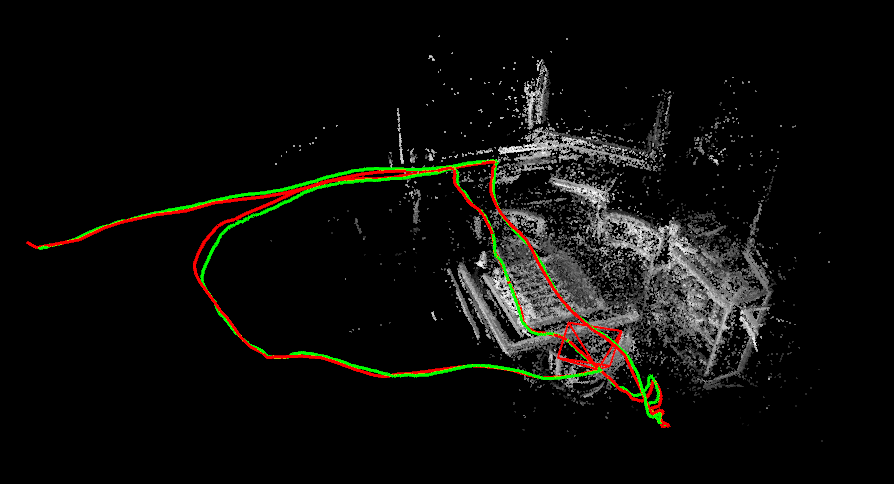
\includegraphics[width = 4.5cm]{experiments/cropped/chess.png}}\quad
	\subfloat[Fire]{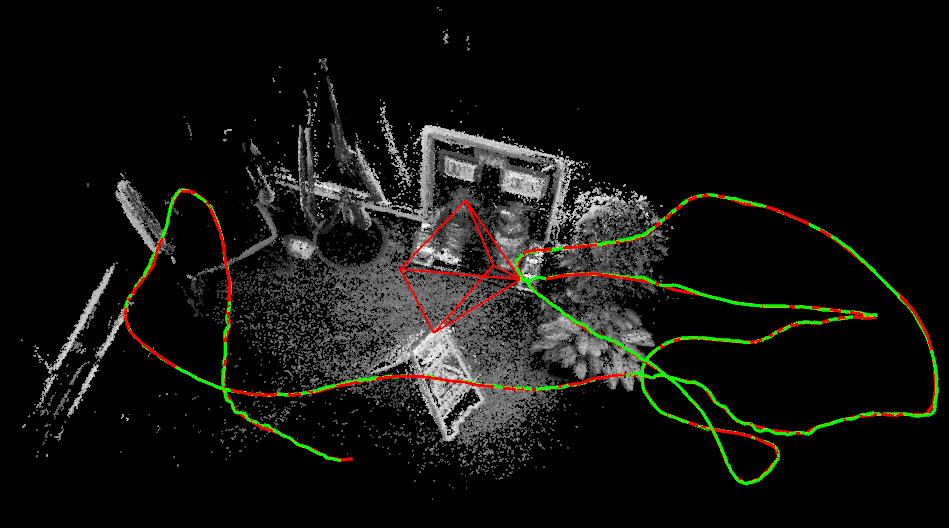
\includegraphics[width = 4.5cm]{experiments/cropped/fire.png}}\quad
	\subfloat[Heads]{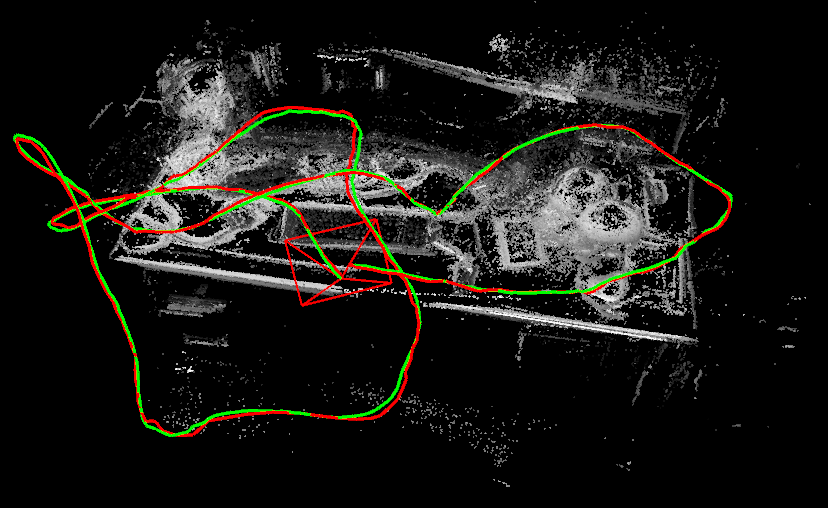
\includegraphics[width = 4.5cm]{experiments/cropped/heads.png}}
	
	\medskip
	
	\subfloat[Office]{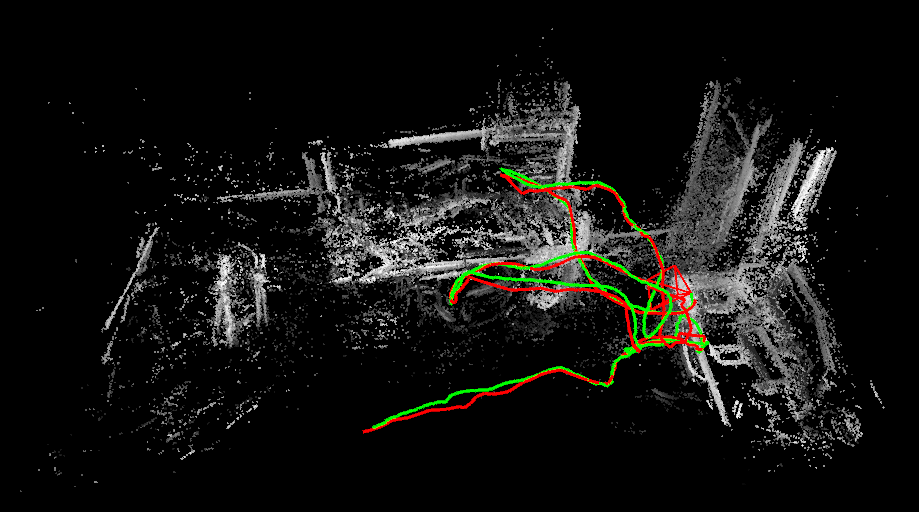
\includegraphics[width = 6cm]{experiments/cropped/office.png}}\quad
	\subfloat[Pumpkin]{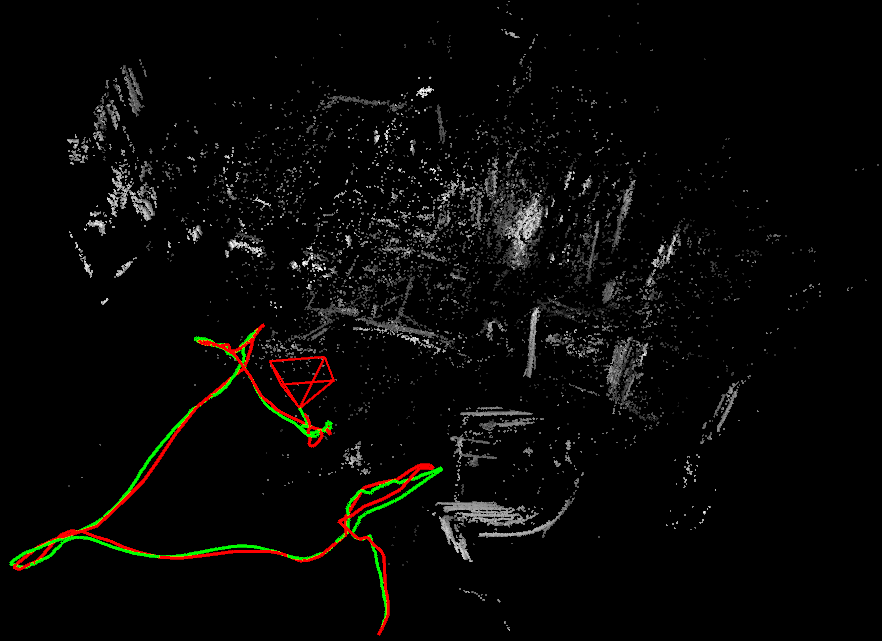
\includegraphics[width = 6cm]{experiments/cropped/pumpkin.png}}
	
	\medskip
	
	\subfloat[Red Kitchen]{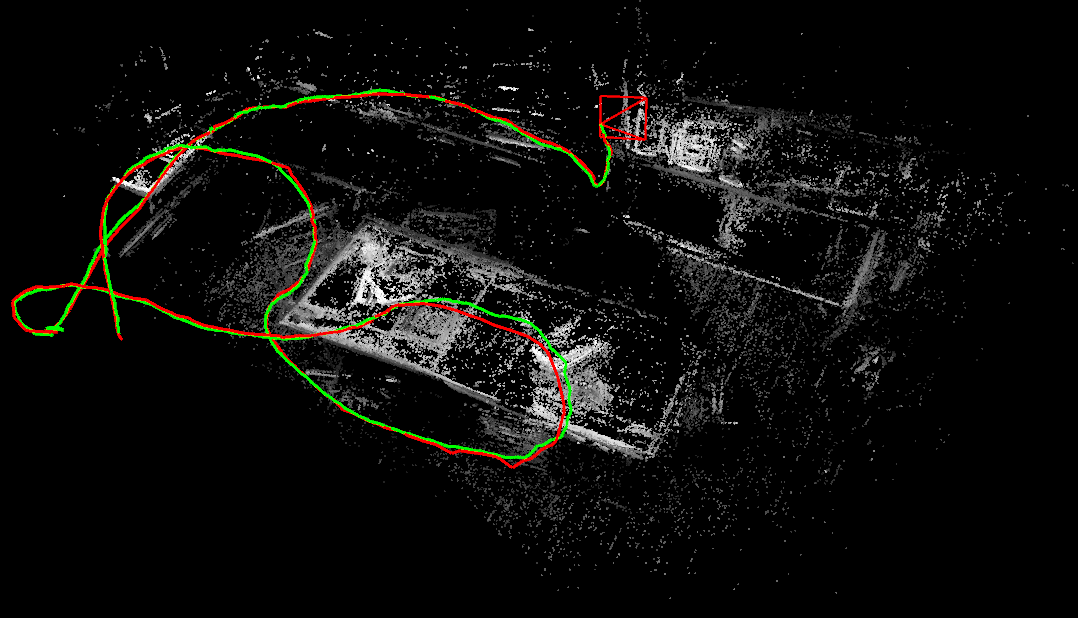
\includegraphics[width = 7cm]{experiments/cropped/redkitchen.png}}\quad
	\subfloat[Stairs]{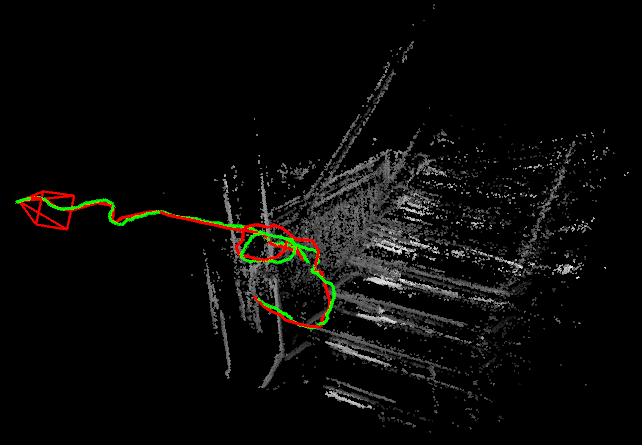
\includegraphics[width = 5cm]{experiments/cropped/stairs.png}}
	
	\caption{Pointcloud representations of 7-Scenes generated by running DSO on a single sequence. The green trajectory represents the ground truth (seeded to the coarse tracker), while the red line connects the further optimized keyframe poses.}
	\label{fig:visualodometry_7scenes}
\end{figure}

\begin{figure}
	\centering
	
	\subfloat[Great Court]{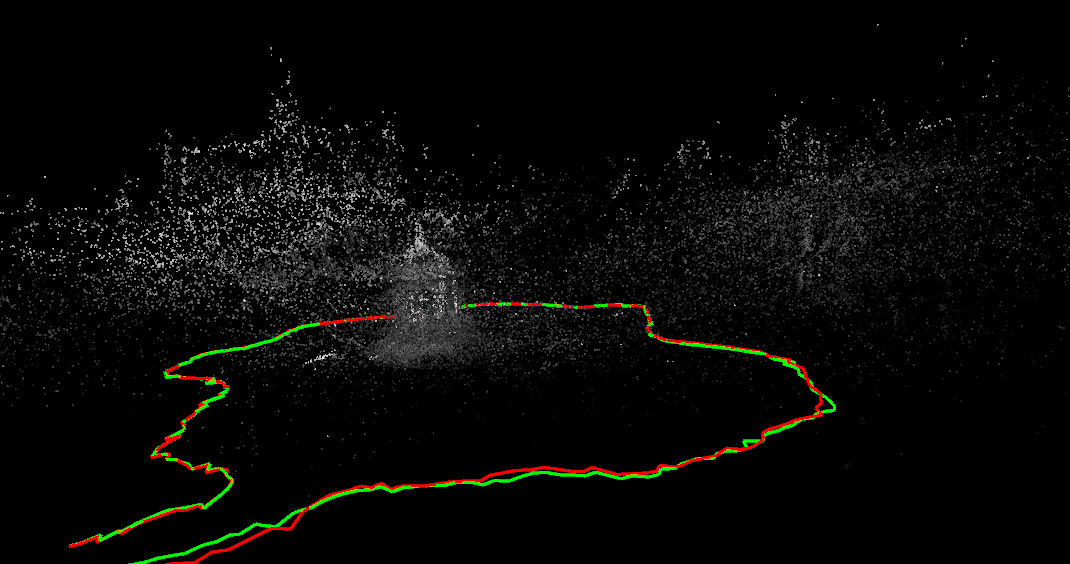
\includegraphics[width = 7cm]{experiments/cropped/greatcourt.png}}\quad
	\subfloat[King's College]{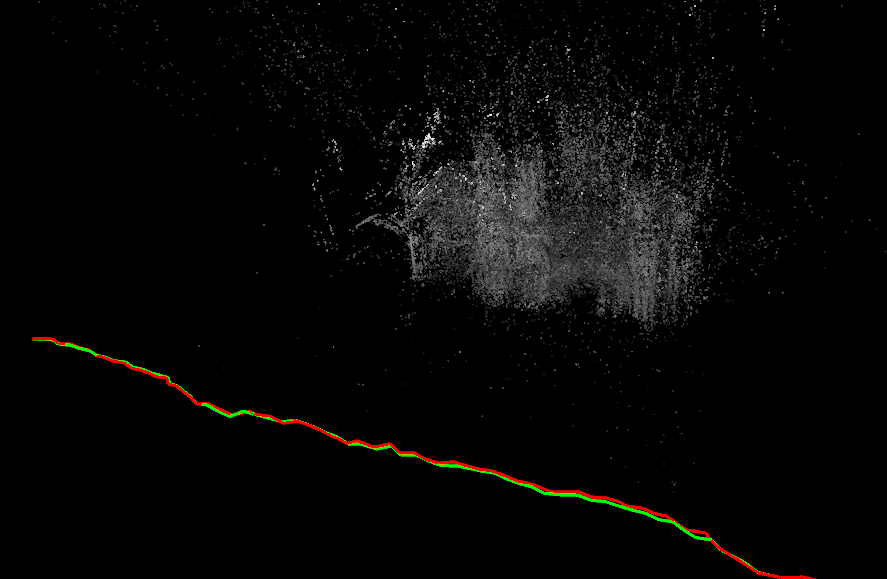
\includegraphics[width = 6cm]{experiments/cropped/kingscollege.png}}
	
	\medskip
	
	\subfloat[Street]{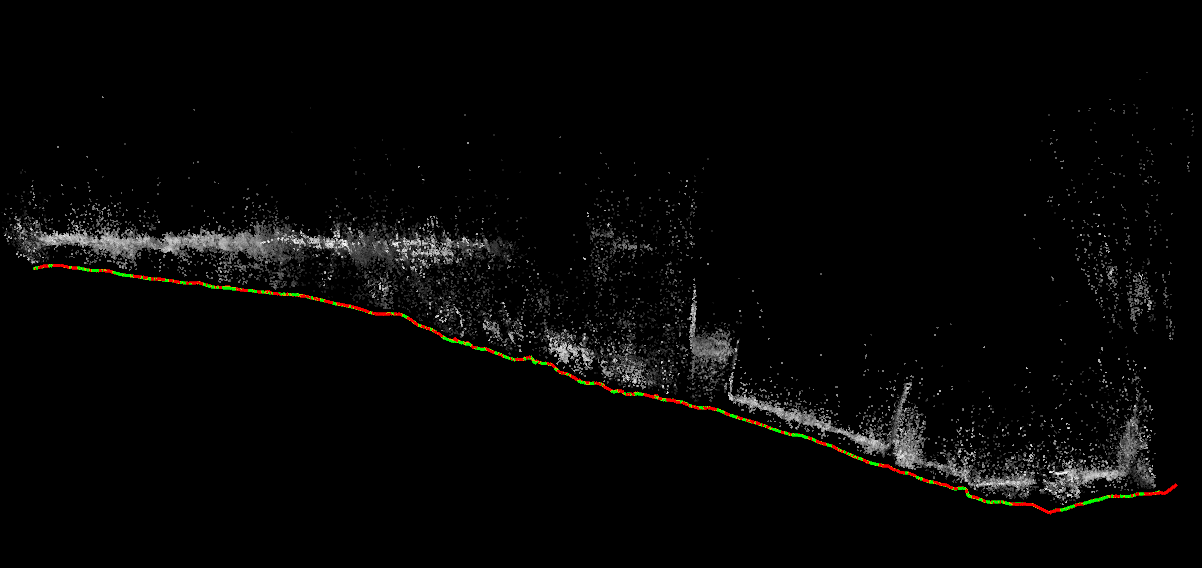
\includegraphics[width = 7cm]{experiments/cropped/street.png}}\quad
	\subfloat[Old Hospital]{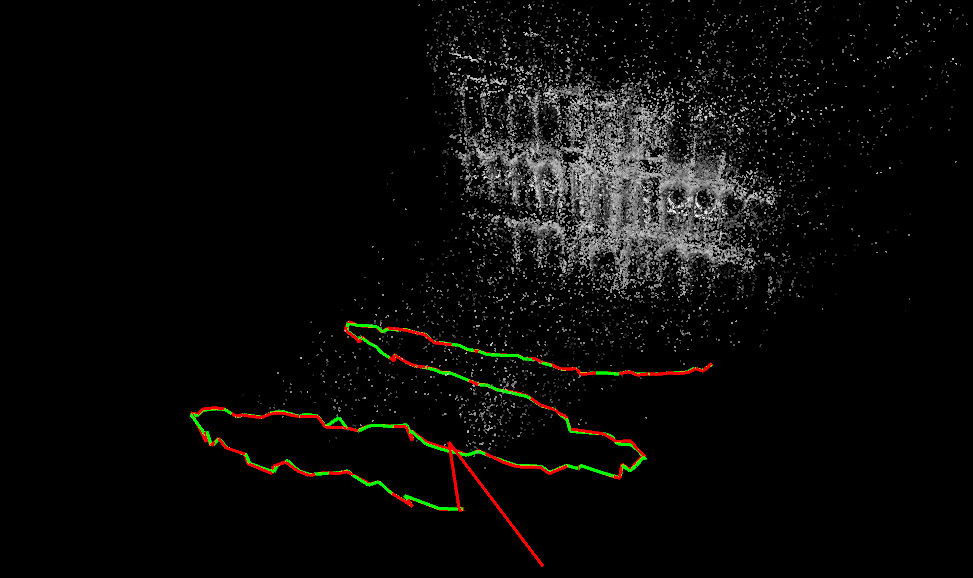
\includegraphics[width = 6cm]{experiments/cropped/oldhospital.png}}
	
	\medskip
	
	\subfloat[Shop Facade]{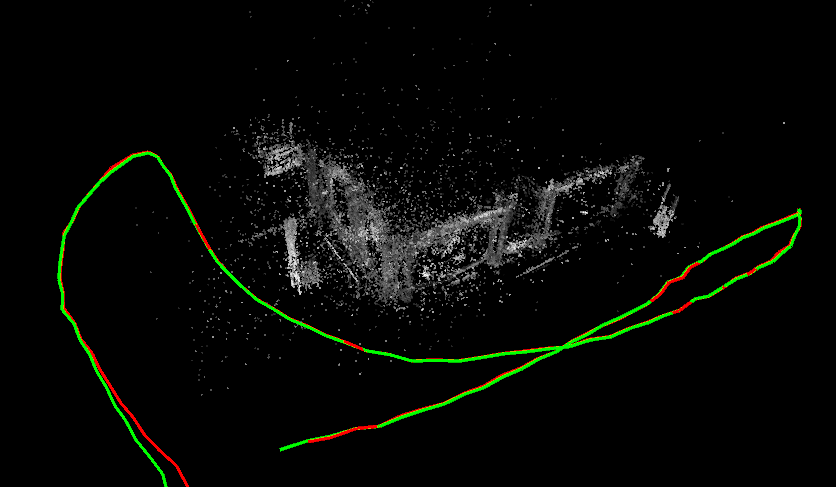
\includegraphics[width = 6cm]{experiments/cropped/shopfacade.png}}\quad
	\subfloat[St Mary's Church]{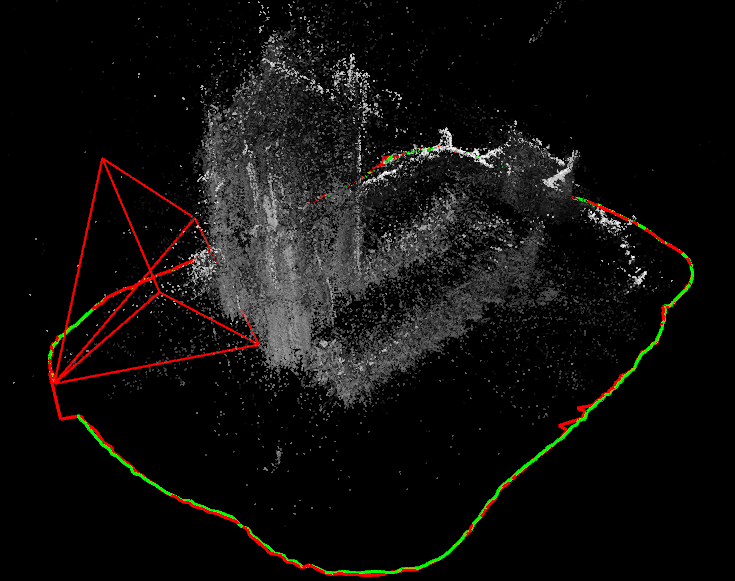
\includegraphics[width = 6cm]{experiments/cropped/stmaryschurch.png}}
	
	\caption{Pointcloud representations of Cambridge Landmarks generated by running DSO on a single sequence. These are urban outdoor scenes, and the scale is an order of magnitude larger than 7-Scenes. Street is nearly 0.4km.}
	\label{fig:visualodometry_cambridge}
\end{figure}

\section{7-Scenes}

To evaluate the method, we used the 7-Scenes dataset introduced by Shotton \textit{et al}.\ \cite{shotton2013scene}. This consists of RGB-D video shot in seven small indoor environments, with spatial extents measuring from 1m$^3$ to 18m$^3$. We aim to achieve high quality results while completely discarding the depth channels, to demonstrate the viability of relocalization using a purely monocular RGB camera with semi-dense depth estimates.

For relocalization, the key requirement is to find a sufficiently close trajectory, since further bundle adjustment should serve to refine the accuracy. For 7-Scenes, ``sufficiently close'' is typically reported having an error of less than 5cm and 5\textdegree for a particular keyframe. In \fref{tab:7scenes-reloc}, we report relocalization accuracy using both SIFT and learned features. Despite the lack of any sort of direct depth-sensing camera, we achieve results that are comparable to prior work with sparse keypoints. In Schmidt \textit{et al}.\ \cite{schmidt2017self}, the authors assume they have access to a fused TSDF model, but we only use the pointcloud that is incrementally published during visual odometry.

As an aside, we note that some of the included scenes are more challenging than others. In particular, Stairs has a large amount of inherent geometric ambiguity in the form of close-up views of a staircase. Some scenes contain objects that are difficult to track, such as shiny, reflective surfaces in Red Kitchen and see-through metal grating in Stairs. Still other scenes contain a large amount of visually similar clutter. We anticipate that further improvement could be made taking into account these repeated geometric and semantic properties.

\begin{table}[h]
	\begin{tabular} { l | c c c c}
		Scene & Sparse RGB \cite{shotton2013scene} & Schmidt \textit{et al}.\ \cite{schmidt2017self} & Semi-Dense SIFT & Semi-Dense Learned \\
		\hline
	Chess       & 70.7\% & 97.75\% & 59.76\% & 11.90\% \\
	Fire        & 49.9\% & 96.55\% & 54.61\% & 10.35\% \\
	Heads       & 67.6\% & 99.8\%  & 63.08\% & 9.90\% \\
	Office      & 36.6\% & 97.2\%  & 28.99\% & 1.85\% \\
	Pumpkin     & 21.3\% & 81.4\%  & 14.88\% & 1.38\% \\
	Red Kitchen & 29.8\% & 93.4\%  & 24.34\% & 1.34\% \\
	Stairs      &  9.2\% & 77.7\%  &  2.28\% & 0.2\% \\
	\end{tabular}
	\caption{Percent of frames localized within 5cm and 5 degrees for the 7-Scenes dataset.}
	\label{tab:7scenes-reloc}
\end{table}

In \fref{tab:7scenes-reloc}, we compare our results to several RGB-D relocalization techniques. Sparse RGB is a baseline presented in \cite{shotton2013scene}, which performs matching similar to our SIFT approach. We note that, without the use of depth-sensing hardware or global bundle adjustment, our SIFT matching performance is similar to previous baselines. In \fref{fig:reloc_7scenes}, we visualize the relocalized poses on the original trajectory.

Contrary to \cite{schmidt2017self}, we find that the learned descriptors are much poorer quality than hand-crafted SIFT descriptors. We explore several possible reasons for this.

\begin{figure}[h]
	\centering
	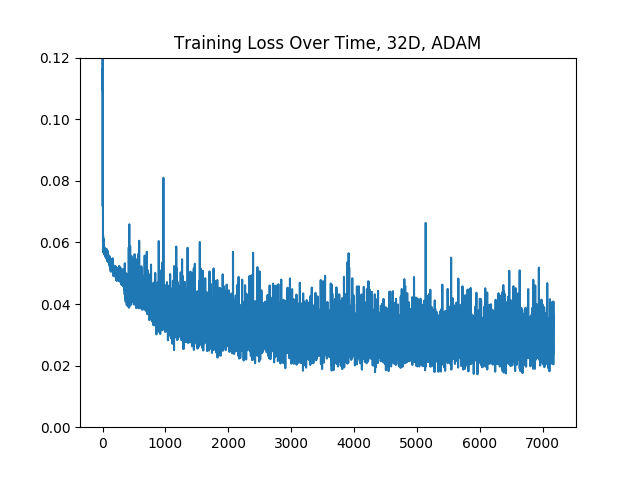
\includegraphics[width=0.8\linewidth]{experiments/trainingiters_32d.png}
	\caption{Loss on the training set over many training iterations. Each training iteration consists of a batch of 12 image pairs, effectively representing tens of thousands of positive samples and millions of negative samples.}
	\label{fig:trainingiters_32d}
\end{figure}

Firstly, we note that the variance in training loss is quite high, as shown in \fref{fig:trainingiters_32d}. This indicates underfitting in the network and could be due to insufficient model complexity to represent the true datapoint correspondences. As this was not a concern in \cite{schmidt2017self}, it may be that our scene pointcloud generated visual odometry is an insufficient replacement for reprojecting a fused 3D model. This could be because the estimated depth maps have too much geometric noise (badly estimated depth pixels), or because our data does not capture the same long-range viewing angle correspondences that are obtainable from a consistent mesh reconstruction (our training correspondences are only gathered from keyframes that were once in the same active window).

Additionally, Schmidt \textit{et al}.\ trained a single network on all the training data in 7-Scenes, whereas we trained 7 networks, one each with the train set of a particular scene. Of course adding more unrelated training data will not reduce underfitting, but it might give a more representative sample of the kind of point correspondences that we would like to detect.

Another consideration is the effect of poor pairwise descriptor correspondences, and for this it is important to recognize the differences between dense and sparse correspondences. For sparse correspondences, we would like to match between few and, generally, fairly distinct points. For dense correspondence, many features may be similar to each other---for example, descriptors evaluated at neighboring pixels will have very close values. The ratio test is intentionally designed to deal with false-positive and true-positive distributions associated with sparse keypoints---for dense keypoints, the distribution changes, and the second nearest neighbor of a point will generally be very close in the descriptor space.

Fortunately, since we have access to ground truth data, we can empirically test how nearest neighbors in the descriptor space are related. In particular, the 7-Scenes dataset provides ground truth poses and fused TSDF volumes (it also contains full depth maps, but these are both uncalibrated and not very precise). We use a freely available marching cubes implementation \cite{ramachandran2011mayavi} to generate an isosurface through the TSDF volume. This gives us a relatively dense mesh of vertices representing a particular scene. Then we proceed by repeatedly sampling two camera poses from the the sequence, and computing descriptors over a semi-dense depth map in the same way as our experimental pipeline. Next, for each descriptor keypoint in the first image, we perform a ray cast from the first camera into the scene, to find a mesh vertex (we use the mesh raycasting implementation of \cite{woop2013embree}, which is quite fast). At this point, the selected vertex may not be visible to the second camera; to check for occlusions, we can project the vertex into the second camera, and then perform a second ray cast back into the scene. If both cameras observe the same vertex (or one a short distance away), the occlusion check passes. In this case, if both cameras have detected a keypoint at their respective reprojected pixels, then we have found a true positive.

Our semi-dense depth maps have 10,000--20,000 points, and even after the occlusion check, we are generally left with around 10,000 truth correspondence between the images. As a result, it is feasible to do an exhaustive matching of all $n^2$ pairwise correspondences, and check their distances. If we consider only one-way nearest neighbors (points in the second image whose descriptors are nearest neighbors to points in the first image), then we can easily check if a true correspondence was the nearest neighbor, or if a very distant match was the nearest neighbor instead. We can also store the distance to the second nearest neighbor, to evaluate the efficacy of the ratio test as a heuristic to prune false positives. In \fref{fig:tpfp_pdf} we do just that. Curiously, the crossing point of the two distributions is still around 0.7, which is the same as the value measured by Lowe \cite{lowe1999object} for SIFT correspondences. However, this only shows the p.d.f.\ of a ratio given the distribution---in actuality, true positives account for only 16\% first nearest neighbor samples, and a large bulk of the true positive distribution does not lie within this p.d.f.. We expect that imposing a higher limit on the confidence of RANSAC would improve this result, but we observe that it also increases the chances of finding a false matches that appear geometrically consistent.

\begin{figure}[h]
	\centering
	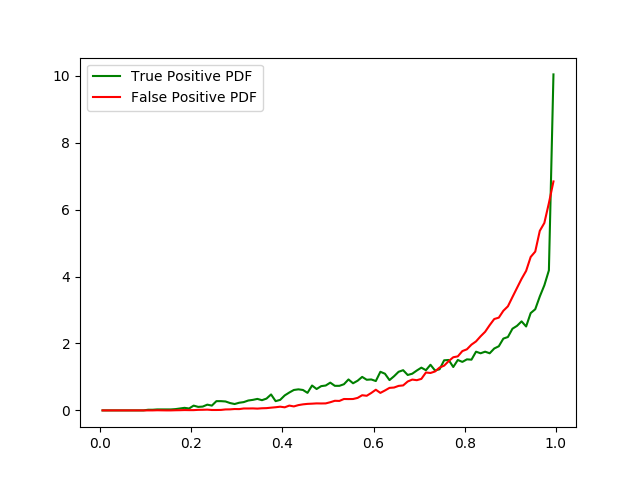
\includegraphics[width=0.8\linewidth]{experiments/tpfp_pdf.png}
	\caption{Estimated probability density function of the ratio between the first nearest neighbor distance and the second nearest neighbor distance for one-way correspondences. The distribution for true positives (the first nearest neighbor is a true correspondence) is shown in green, and for false positives (the first nearest neighbor is a false correspondence) is shown in red.}
	\label{fig:tpfp_pdf}
\end{figure}

Finally, we mention that in our work, the sparsity of the correspondences is a direct function of the number of keypoints output from DSO. For our SIFT method, we set this value relatively low---around 2,000 tracked keypoints per frame---and we find that increasing the number to around 20,000 diminishes relocalization rates (by about 10\% on fire, for example). In contrast, our dense descriptors do not vary so much with this change.

In \fref{tab:7scenes-fire-alt}, we address some of these concerns by evaluating on the \textit{fire} scene. In the first three rows, we adjust the ratio used for the ratio test; much lower ratios remove almost all correspondences. Notably, the first entry \textit{Dense $r=1.0$} contains the default model from which all the subsequence models are derived. In the next grouping, we perform the same thresholding comparison, but using the somewhat sparser depth maps used during the SIFT evaluations. The last group experiments with different network settings: \textit{All} used the training data from every scene, and \textit{All-48} used the training data from every scene and was configured to output a 48-dimensional descriptor. In \textit{Semidense-only}, we modify the sampling step of training. Normally, once we have a positive training sample, we sample a negative correspondence from anywhere in the second training image; instead, in the \textit{Semidense-only} sampling strategy, we only select a negative training sample if it also occurred in a semi-dense depth map in the second image. In this way, we discard training samples on low-texture surfaces (which are useless to us anyway) and instead focus training on salient points. Furthermore, \fref{fig:obs-vis} shows a visualized 3D image with the previous sampling method, which is why we think shows promise.

None of these methods showed consistent improvement, so we expect this is a topic for future study.

\begin{table}[h]
	\begin{tabular} { l | c c c}
		Method & Accuracy & Median Translation Error & Median Rotation Error \\
		\hline
		Dense $r=1.0$  & 10.35\% & 20.3cm & 3.62\textdegree \\
		Dense $r=0.99$ & 9.70\% & 18.6cm  & 3.43\textdegree \\
		Dense $r=0.95$ & 11.50\% & 18.1cm & 3.26\textdegree \\
		\hline
		Sparse $r=1.0$   & 5.43\% & 27.3cm & 4.83\textdegree \\
		Sparse $r=0.99$  & 5.22\% & 27.4cm & 4.75\textdegree \\
		\hline
		All            & 23.00\% & 10.8cm & 2.03\textdegree \\
		All-48         & 0.95\% &  62.3cm & 11.7\textdegree \\
		Semidense-only & 10.95\% & 22.1cm & 4.27\textdegree \\
	\end{tabular}
	\caption{Relocalization accuracy (percent \textless5cm, \textless5\textdegree), plus median error in translation and in rotation in \textit{fire}.}
	\label{tab:7scenes-fire-alt}
\end{table}


\begin{figure}
	\centering
	
	\subfloat[Default]{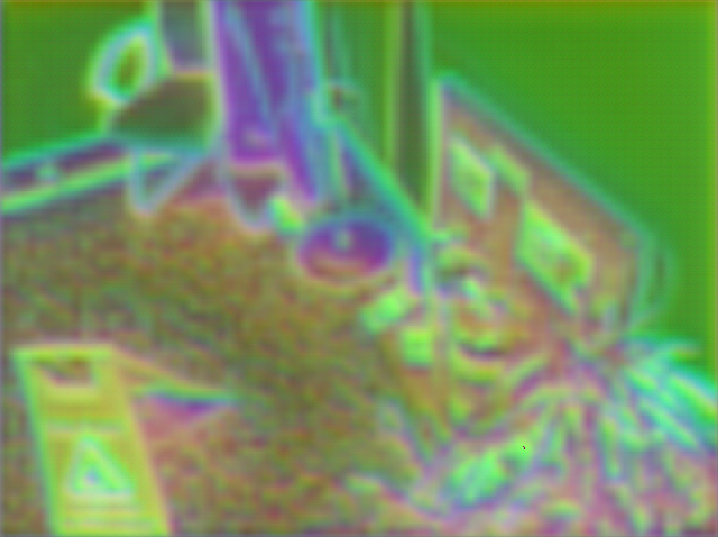
\includegraphics[width = 6cm]{experiments/sample_default.png}}\quad
	\subfloat[Semidense Only]{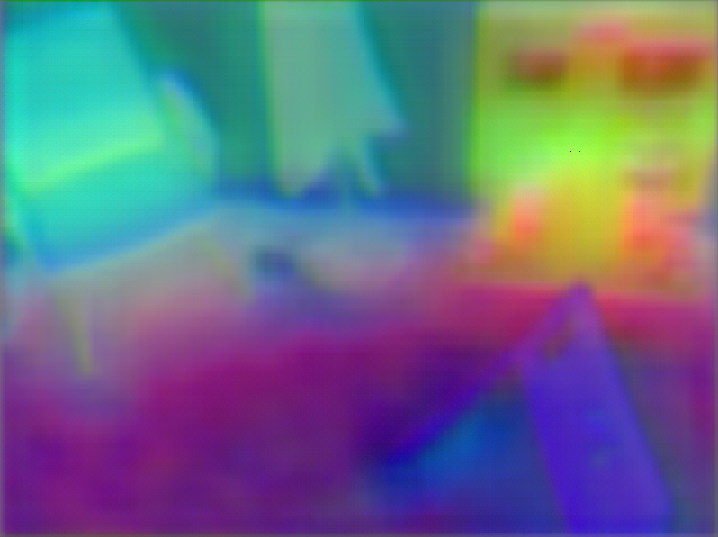
\includegraphics[width = 6cm]{experiments/sample_focused.png}}
	\caption{Visualization of descriptors from two views using different sampling strategies for training. In the default strategy, edges are very visually distinct from object interiors, whereas in the second strategy, they are more visually distinct from each other.}
	\label{fig:obs-vis}
\end{figure}

\begin{figure}
	\centering
	
	\subfloat[Chess]{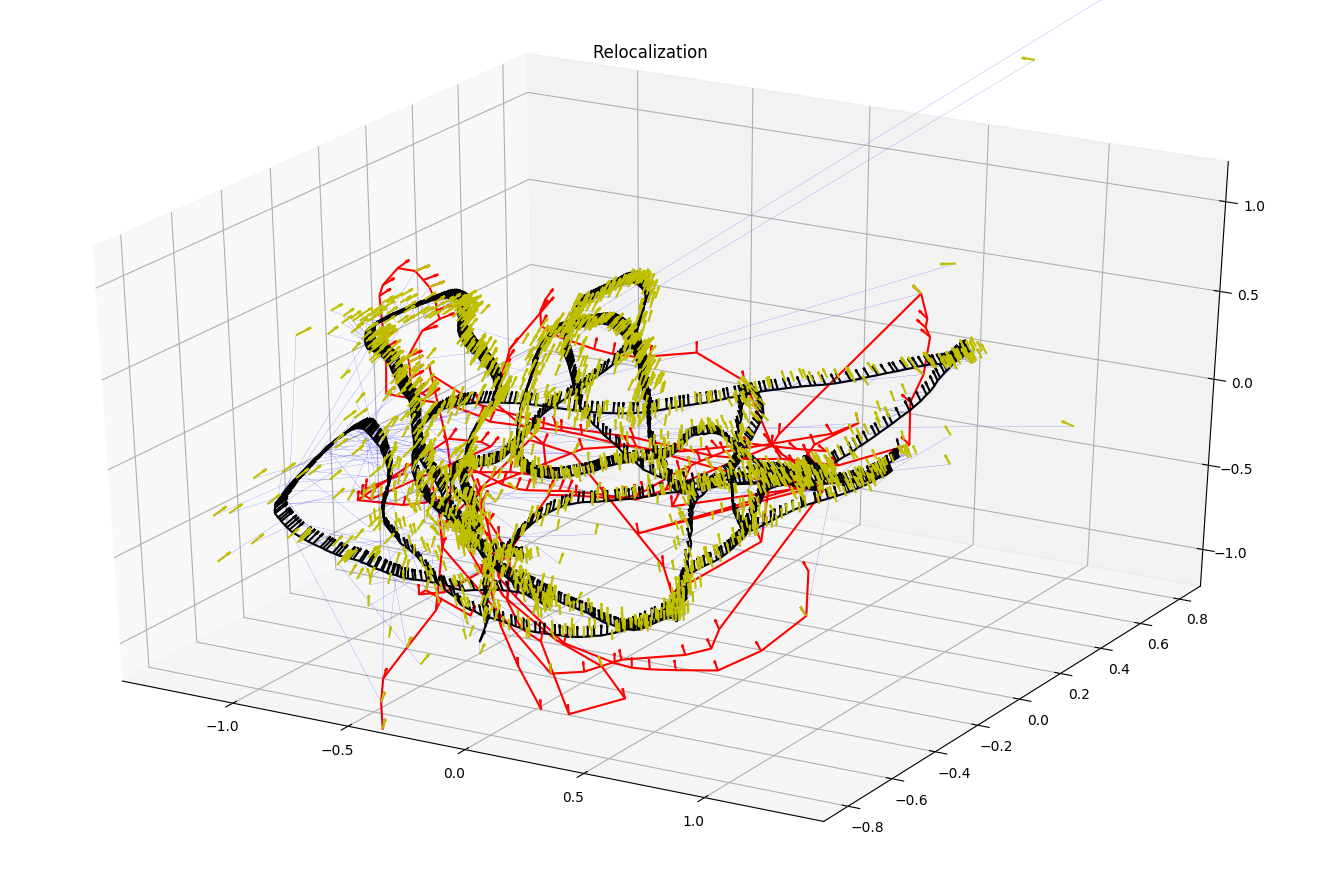
\includegraphics[width = 6cm]{experiments/reloc/chess.png}}\quad
	\subfloat[Fire]{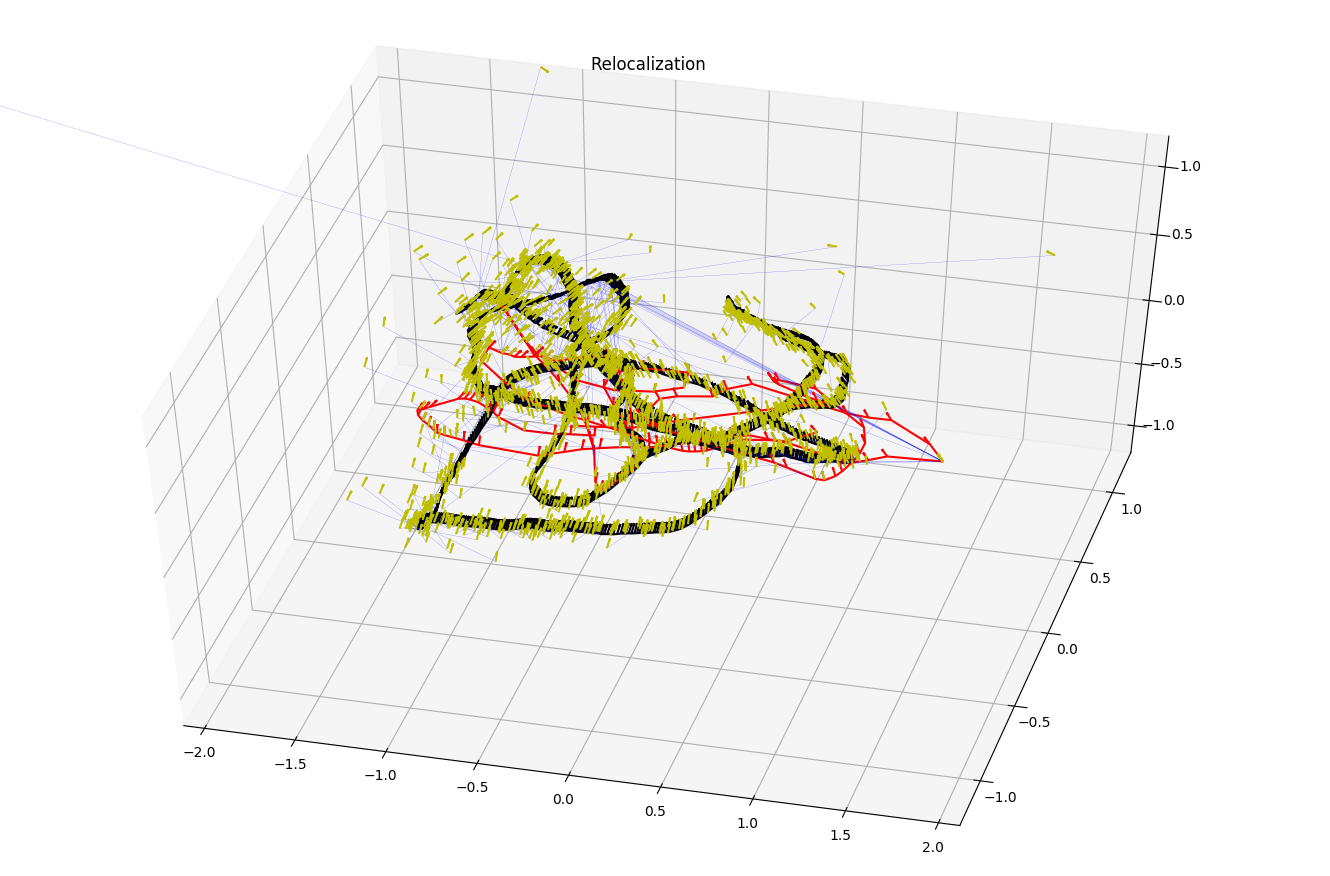
\includegraphics[width = 6cm]{experiments/reloc/fire.png}}
	
	\medskip
	
	\subfloat[Heads]{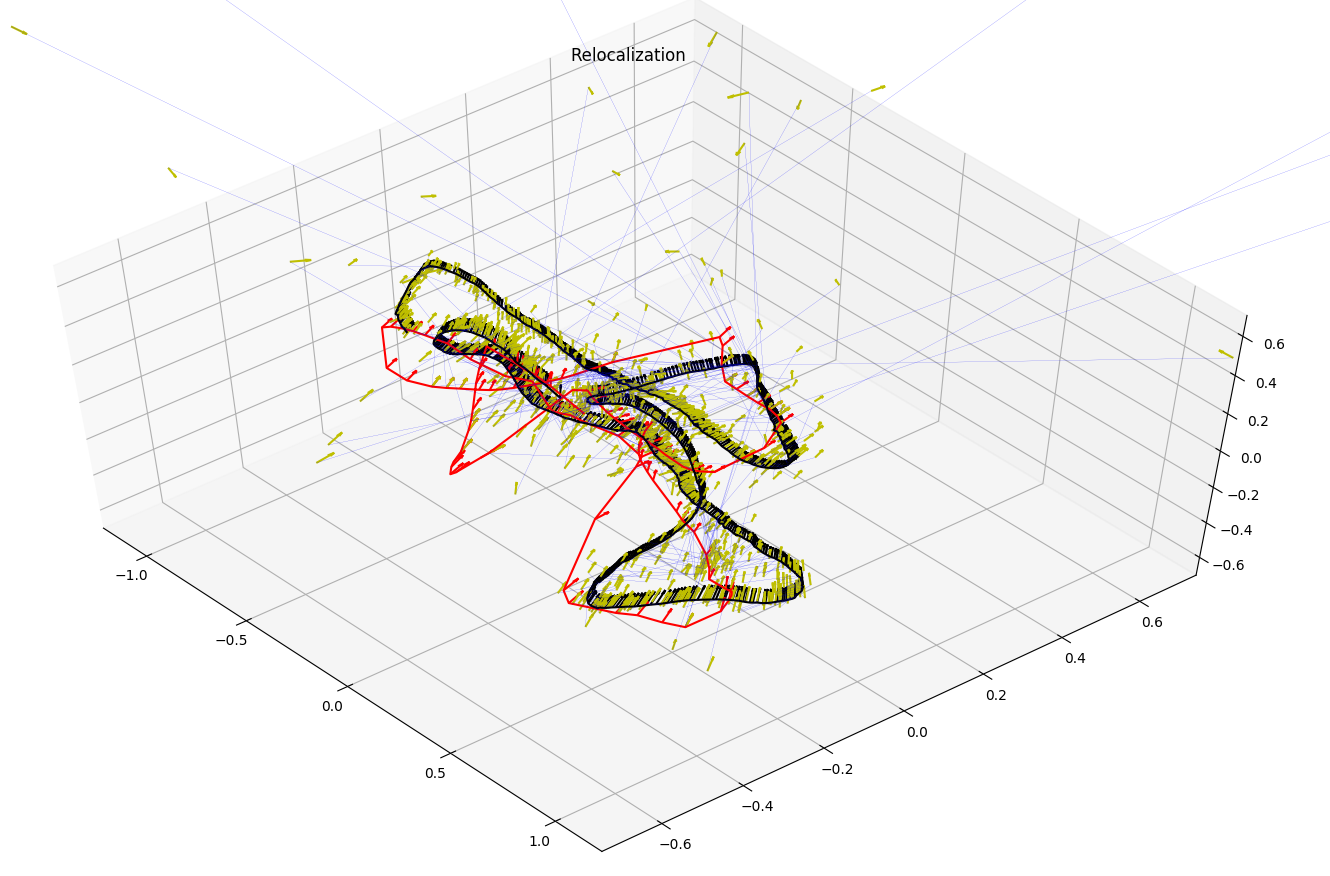
\includegraphics[width = 6cm]{experiments/reloc/heads.png}}\quad
	\subfloat[Office]{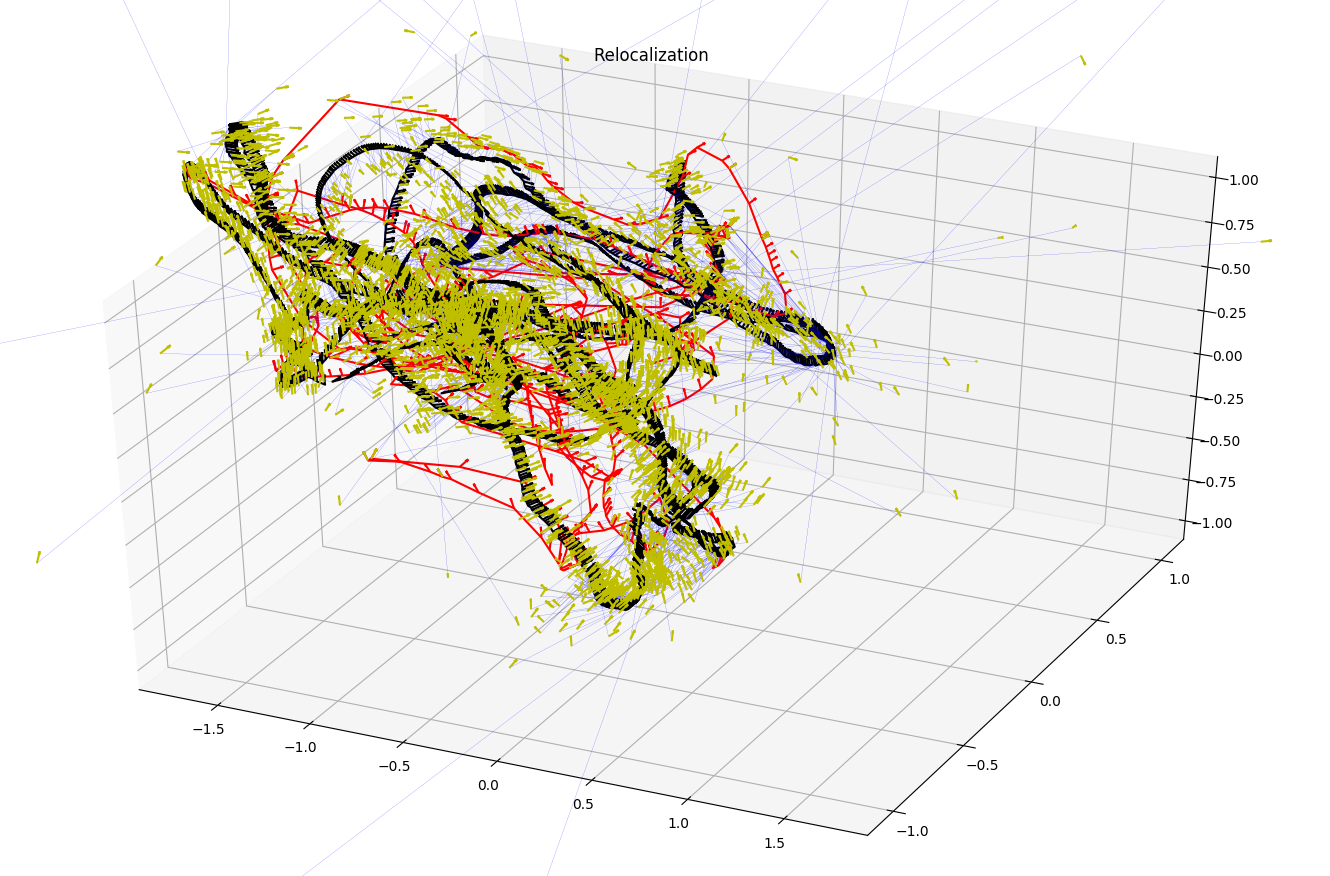
\includegraphics[width = 6cm]{experiments/reloc/office.png}}
	
	\medskip
	
	\subfloat[Pumpkin]{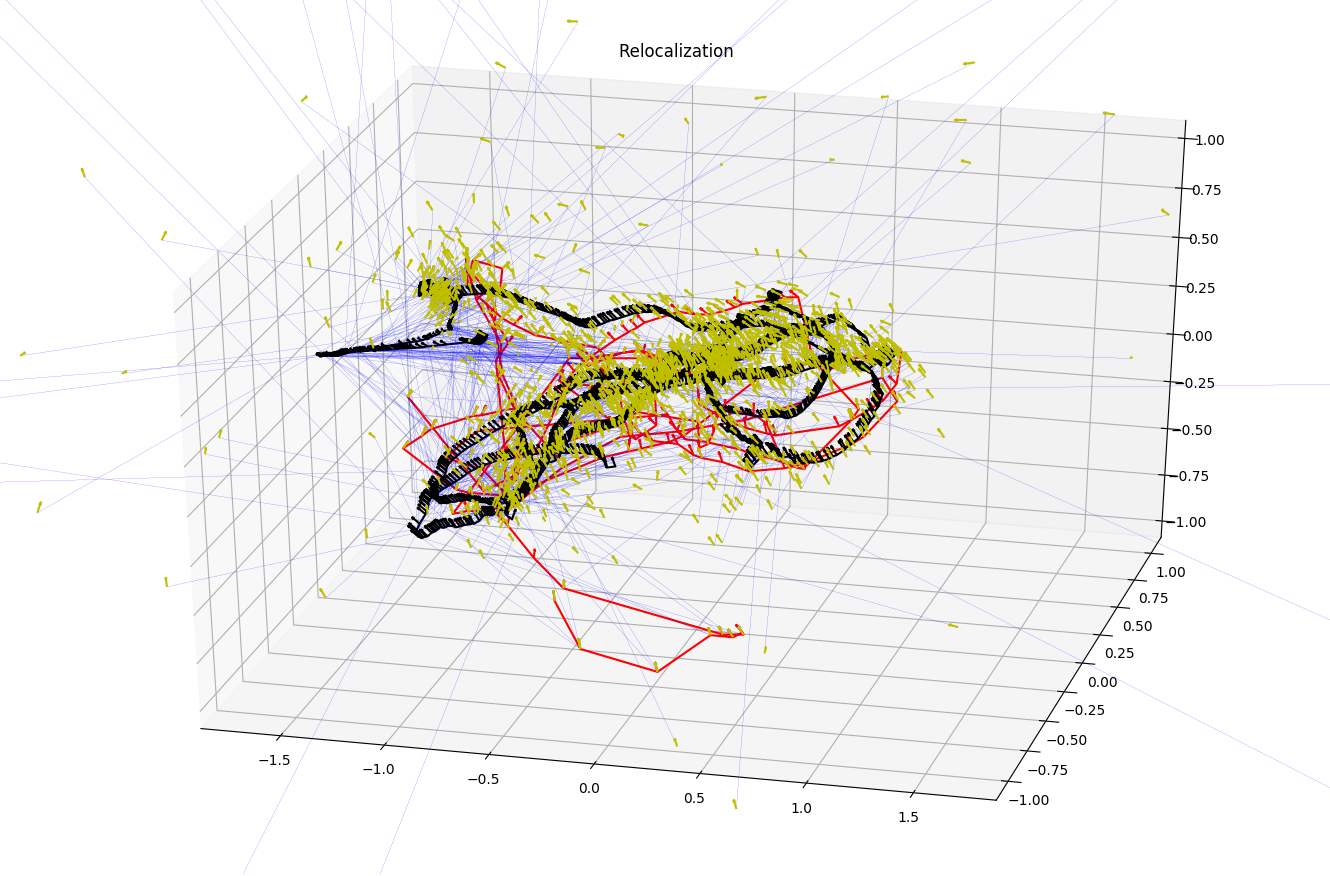
\includegraphics[width = 6cm]{experiments/reloc/pumpkin.png}}\quad
	\subfloat[Red Kitchen]{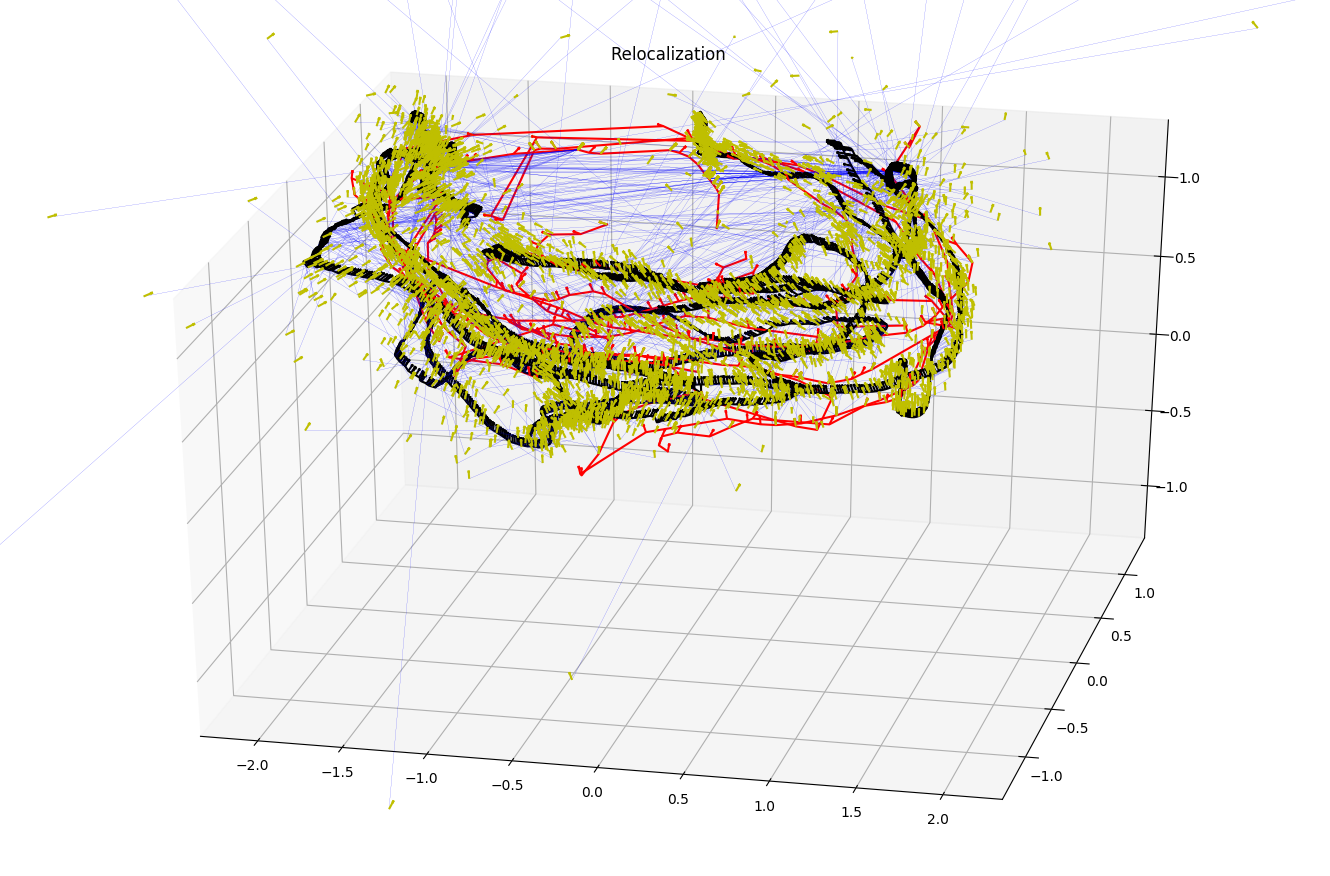
\includegraphics[width = 6cm]{experiments/reloc/redkitchen.png}}
	
	\medskip
	
	\subfloat[Stairs]{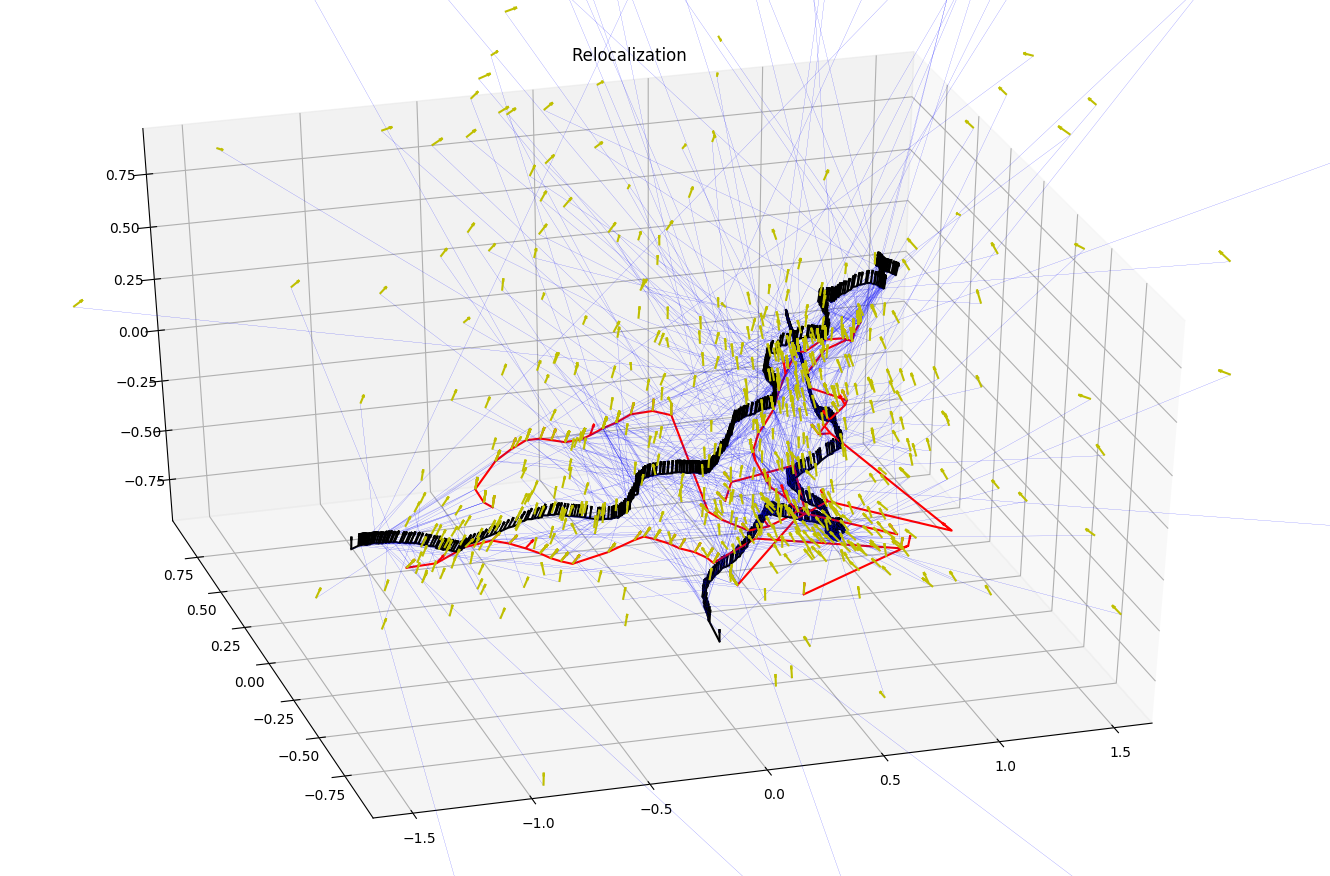
\includegraphics[width =  6cm]{experiments/reloc/stairs.png}}
	
	\caption{Relocalized trajectories using SIFT descriptors for each of 7-Scenes. Here, yellow represents the relocalized test poses, black represents the unknown ground truth of the test poses, and red indicates the poses extracted from visual odometry, as seen earlier. A blue line is drawn between each estimated pose and its true correspondence in the ground truth.}
	\label{fig:reloc_7scenes}
\end{figure}

\section{Cambridge Landmarks}

The authors of \cite{kendall2015posenet} also provide a relocalization benchmarking dataset. Their dataset consists of RGB videos and ground truth measurements of a hand-held camera traveling around outdoor urban landmarks. The lack of a depth sensor prevents the use of state-of-the-art RGB-D relocalization approaches. This dataset also has several other challenging aspects, which we enumerate here:
\begin{itemize}
	\item Consecutive frames of the dataset contain large purely rotational movements, making it difficult to estimate depth of newly observed points.
	\item The recorded video has large changes in exposure between frames due to changing illumination conditions, ranging from panning through shadows to literally staring at the sun.
	\item The camera movement is shaky and has large geometric distortions due to a rolling shutter. The original videos are also subsampled from 30 frames per second to around 2 frames per second.
	\item The ground truth data contains erroneous measurements, making it only mostly reliable for train set initialization.
\end{itemize}

In our experiments, we rescale the images from 1920x1080 to 768x416, both so that visual odometry can be performed quickly and in order to not exceed GPU memory limits for our learned descriptor. This dataset also does not contain camera calibration, but we estimate the camera distortion parameters using an incremental SfM framework with a camera model optimization \cite{schoenberger2016sfm} \cite{schoenberger2016mvs} \cite{schoenberger2016vote}. We found modeling the camera with second-degree radial tangential distortion worked best.

We compare our results in \fref{tab:cambridge-reloc} to the results of Kendall \textit{et al}.\ \cite{kendall2015posenet}, in the form of median translation and rotation error per frame per scene. The original authors sought to directly regress on the 6-DoF pose of the camera, in order to mimic the action of human neuronal localization patterns. This helps to give a coarse estimate and prevent degenerate pose estimates (in which the predicted pose lies well outside the scene due to incorrect matching), since the original network is never trained on poses outside the scene. However, it requires a source of ground truth for training, whereas our method relies only on the local coordinate frames computed in each visual odometry session---we can re-align our predicted results as desired. We furthermore suspect that performing more exhaustive robust pose estimation and refinement is necessary to achieve the high accuracy demonstrated in other state-of-the-art relocalization results.

\begin{table}[h]
	\begin{tabular} { l | c c c c}
		Scene & PoseNet \cite{kendall2015posenet} & Semi-Dense SIFT & Semi-Dense Learned \\
		\hline
		Great Court      & N/A                    & 1.24m, 0.39\textdegree & 129m, 44.5\textdegree \\
		King's College   & 3.34m, 2.96\textdegree & 2.31m, 1.58\textdegree & 21.8m, 21.5\textdegree \\
		Street           & 1.95m, 4.51\textdegree & 110m, 48.7\textdegree  & 200m, 58.1\textdegree \\
		Old Hospital     & 5.38m, 4.51\textdegree & 16.2m, 14.4\textdegree & 42.3m, 53.6\textdegree \\
		Shop Facade      & 2.10m, 5.20\textdegree & 9.82m, 23.2\textdegree & 19.0m, 49.0\textdegree \\
		St Mary's Church & 4.48m, 5.65\textdegree & 0.47m, 0.72\textdegree & 47.9m, 61.2\textdegree \\
	\end{tabular}
	\caption{Median translation and rotation error for relocalized frames in the Cambridge Landmarks dataset.}
	\label{tab:cambridge-reloc}
\end{table}

\cleardoublepage

